\chapter{Исследовательская часть}

В данном разделе будут приведены результаты работы разработанного программного обеспечения и поставлен эксперимент по сравнению уровня и характера шума синтезируемого изображения с использование классическом алгоритма (метода Монте - Карло) и квантового алгоритма избыточной выборки на различных размерах изображения.

\section{Результаты работы программного обеспечения}

% 3, 4, 5
На изображении \ref{img:example_01} приведен результат работы программы с размером синтезируемого изображения 512x512 пикселей и при использовании 4 итераций увеличения комплексной амплитуды. 

\begin{figure}[H]
	\begin{center}
		%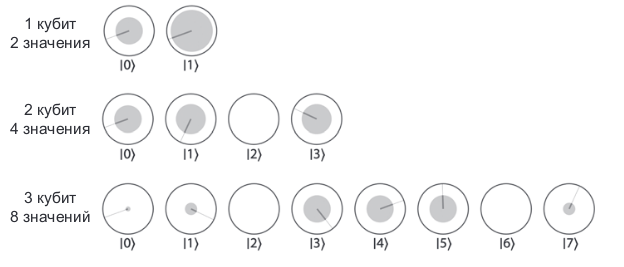
\includegraphics[scale=0.7]{img/qint.png}
	\end{center}
	\captionsetup{justification=centering}
	\caption{Результаты работы ПО с размером синтезируемого изображения 512х512 и использования 4 итераций увеличения комплексной амплитуды}
	\label{img:example_01}
\end{figure}

На рисунке \ref{img:example_02} представленно тоже самое изображение, но уже при использовании 8 итераций увеличения комплексной амплитуды. 

\begin{figure}[H]
	\begin{center}
		%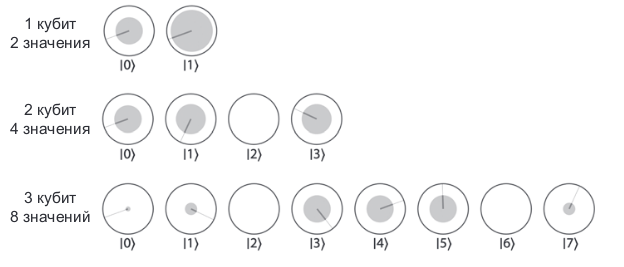
\includegraphics[scale=0.7]{img/qint.png}
	\end{center}
	\captionsetup{justification=centering}
	\caption{Результаты работы ПО с размером синтезируемого изображения 512х512 и использования 8 итераций увеличения комплексной амплитуды}
	\label{img:example_02}
\end{figure}

\begin{figure}[H]
	\begin{center}
		%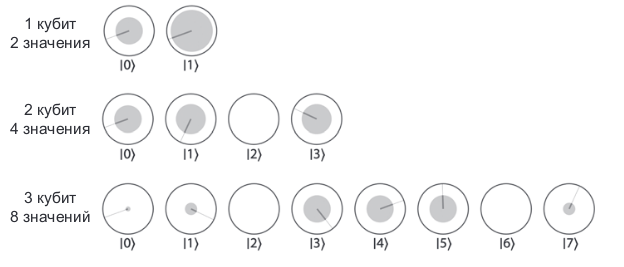
\includegraphics[scale=0.7]{img/qint.png}
	\end{center}
	\captionsetup{justification=centering}
	\caption{Результаты работы ПО с размером синтезируемого изображения 1024х1024 и использования 4 итераций увеличения комплексной амплитуды}
	\label{img:example_03}
\end{figure}

На риснуке \ref{img:example_03} представлен результат работы программы при синтезе изображения размером 1024х1024 пикселя и при использовании 4 итераций усиления комплексной амплитуды.

\section{Постановка эксперимента} 

\subsection{Цель эксперимента}

Целью эксперимента является проведение сравнения уровня и характера зашумлённости изображения синтезируемого классическим алгоритмом избыточной выборки (алгоритм Монте-Карло) и алгоритмом квантовой избыточной выборки.

\subsection{Описание эксперимента}

Сравнить уровень зашумленности двух синтезируемых изображений можно расчитав средний процент ошибки на каждый пиксель.

Результаты сравнения уровня зашумлённости для изображений разных размеров приведены в таблице 4.1. Во втором и третьем столбце таблицы расположены средние проценты ошибок для рассматриваемых реализаций алгоритмов. Размер сабпикселя равен 4х4.

\begin{table}[h!]
	\label{tab:noise}
	\caption{Сравнение уровня зашумленности для классического и квантового алгоритма избыточной выборки.}
	\begin{center}
		\begin{tabular}{|c | c | c|} 
			\hline
			Размер изображения & Классическая выборка & Квантовая выборка \\  
			\hline
			64x64 & 3\% & 2\%  \\
			\hline
			128x128 & 4\% & 2\% \\
			\hline
			256x256 & 4\% & 3\% \\
			\hline
			512x512 & 4\% & 3\% \\
			\hline
			1024x1024 & X\%  & X\% \\
			\hline
		\end{tabular}
	\end{center}
\end{table}

Из-за того что в квантовом случае пиксели получаемого изображения могут быть либо идеальными, либо крайне зашумленными \cite{PQC-classic}, сравнение характера шума  изображения можно провести подсчитав процент идеальный пикселей от всего изображения. 
% почему-то не работает ref но мне ща лень разбираться
В таблице \ref{tab:noise_02} приведено сравнение характера шума для разных размеров изображения. Размер сабпикселя равен 4х4.

\begin{table}[h!]
	\label{tab:noise_02}
	\caption{Сравнение характера шума классического и квантового алгоритма избыточной выборки.}
	\begin{center}
		\begin{tabular}{|c| c | c|} 
			\hline
			Размер изображения & Классическая выборка & Квантовая выборка \\  
			\hline
			64x64 & 58\% & 88\%  \\
			\hline
			128x128 & 71\% & 78\% \\
			\hline
			256x256 & 63\% & 75\% \\
			\hline
			512x512 & 62\% & 73\% \\
			\hline
			1024x1024 & X\% & X\% \\
			\hline
		\end{tabular}
	\end{center}
\end{table}


\section*{Вывод}

Как и ожидалось, уровень зашумленности изображения примерно равен как для классической выборки, так и для квантовой. Так, например, средний процент ошибки на пиксель при размере синтезируемого изображения 512х512 для квантового алгоритма составляет 3\%, а для классического 4\% соотвественно.

Квантовая выборка на маленьких размерах изображения выдает большой процент идеальных пикселей. Например, для изображения размером 64х64 количество идеальных пикселей составляет 88\% от всего изображения. Но, с увеличением изображения этот процент незначительно падает, и уже на размере изображения 512х512 составляет 73\%. Несмотря на это, классическая выборка даже в самом лучшем случае не добивается такого результата -- ее лучший результат 71\% идеальных пикселей для размера изображения 128х128. Квантовый алгоритм генерирует на 10\%..30\% идеальных пикселей больше, чем его классический аналог, из чего можно сделать вывод о сильных различиях в характере шума.